\section{O processo: Test-Driven Security com red e blue team}
\label{sec:processo}

Os artefatos de processo descrevem como os ciclos rodam na prática: o ciclo em si (\texttt{docs/05-tds-process.md}); o plano das iterações, com calendário, ritual, regras de engajamento e medição de custo (\texttt{docs/06-plano-iteracoes.md}); o passo a passo do red team (\texttt{docs/07-guia-red-team.md}); e o fluxo de branches e de pull requests (\texttt{CONTRIBUTING.md}). Juntos, eles são a parte mais reutilizável do trabalho: nada neles depende de neurofeedback.

\subsection{O ciclo}

O ciclo tem quatro momentos. O primeiro é a \textbf{modelagem}, feita uma vez: o STRIDE sobre o fluxo de dados deriva as histórias, cada história vira uma árvore, e cada folha vira um teste. O segundo é a \textbf{build 0}, o aplicativo sem controles, de propósito, como linha de base; quase todas as folhas ficam abertas. O terceiro é a \textbf{iteração}, repetida: o red ataca a build atual seguindo as árvores; cada ataque com sucesso vira uma issue com evidência; o blue implementa o controle num pull request que inclui o teste de regressão; e o teste passa a rodar em todo build futuro. O quarto é o \textbf{fim}, quando o custo de fechar as folhas restantes passa do valor de fechá-las. No MATE sempre sobra folha aberta, e isso é documentado como conclusão, não como fracasso.

Os papéis são dois: o blue team construiu as builds e os controles, e o red team atacou e manteve as árvores e os casos de abuso. A regra de ouro do repositório resume a disciplina: nenhuma defesa entra na \texttt{main} sem o teste de regressão correspondente, porque segurança é regra da esteira, não disciplina individual. Controles estruturais, como hardkey, servidor de ativação ou o algoritmo no servidor, são avaliados como experimentos numa branch \texttt{hipotese/<nome>}: o blue implementa, o red ataca a branch, e só sobe para a \texttt{main} o que se prova. As demais branches seguem o mesmo vocabulário: \texttt{fix/<folha>} para as correções do blue e \texttt{ataque/<folha>} para os testes do red.

\subsection{Como um ataque vira teste sem travar a main}

No MATE sempre sobra folha aberta. Se o teste de uma folha aberta simplesmente falhasse, a esteira nunca ficaria verde e a proteção de branch travaria a \texttt{main} para sempre. Por isso cada folha tem um estado declarado em \texttt{security-tests/estado-folhas.json}, e cada teste compara o resultado do ataque com esse estado, como mostra o Quadro~\ref{qd:estado}.

\begin{table}[htbp]
\centering
\caption{O teste compara o resultado do ataque com o estado declarado da folha.}
\label{qd:estado}
\small
\begin{tabular}{L{2.8cm}L{2.6cm}L{2.2cm}L{6.4cm}}
\toprule
Estado declarado & O ataque & Esteira & Significado \\
\midrule
aberta & funcionou & verde & buraco conhecido e documentado \\
aberta & falhou & vermelha & a folha fechou: atualizar o estado e a matriz \\
fechada & falhou & verde & o controle resiste \\
fechada & funcionou & vermelha & regressão: o merge é barrado \\
\bottomrule
\end{tabular}
\end{table}

O desenvolvimento guiado por testes acontece em quatro passos. O red sobe o teste com a folha \texttt{aberta}: a esteira fica verde e o buraco fica registrado. O blue abre uma branch \texttt{fix/<folha>}, cujo primeiro commit muda a folha para \texttt{fechada}, e a esteira fica vermelha. O controle entra, e a esteira volta ao verde. Depois do merge, se a folha reabrir em qualquer build, a esteira acusa a regressão.

Dois cuidados impedem resultados enganosos. O primeiro é o \textbf{controle positivo}: antes de cada ataque, o teste confirma que o aplicativo original recusa sem licença e abre o treino com uma licença legítima. A partir da v1, essa licença é emitida na hora para a máquina que roda a suíte, com a chave privada do fornecedor guardada como segredo da esteira; sem a chave, fora da esteira, o controle fica parcial. Se o controle positivo falhar, o resultado é inconclusivo, nunca \texttt{fechada}: um build quebrado que nem abre não pode parecer seguro. O segundo é a \textbf{observação de fora}: o teste observa o aplicativo como o atacante observaria, rodando o executável e verificando se a janela principal abriu e, desde a v2, se continuou aberta durante 30 segundos. Não existe flag ou modo de teste dentro do binário, que seria superfície de ataque a mais.

\subsection{A suíte de testes de ataque}

A suíte (\texttt{security-tests/}) é um projeto xunit.v3 em C\#, com a biblioteca dnlib, a mesma de manipulação de assembly do dnSpy, para os patches. Cada teste é um procedimento repetível com resultado passa ou falha: executa a técnica da folha contra uma cópia do zip da release, observa de fora e compara com o estado declarado. O harness tem quatro peças: \texttt{Alvo.cs} extrai o zip, dá uma cópia descartável por teste, roda e observa o aplicativo; \texttt{EstadoFolhas.cs} compara o resultado com o estado declarado; \texttt{ControlePositivo.cs} garante que o alvo original funciona; e \texttt{Assembleia.cs} abre, altera e grava um assembly. O que o atacante sabe do alvo, como nomes e offsets, vem da tentativa em caixa preta e fica no teste, não no harness. O ponto de entrada é o \texttt{run-all.ps1}, o mesmo na esteira e na máquina de cada um.

Ao fim das cinco builds, a suíte tinha 13 testes de ataque, além do controle positivo: T-F1.1, T-F1.2, T-F1.3, T-F2.2, T-F3.1, T-F3.2 e T-F3.3 (estes dois também na forma da v1), T-H1.1, T-H1.2, T-H2.1 e T-H2.2. As folhas F2.1 (depurador) e F2.3 (edição de memória) foram medidas na mão, porque são difíceis de automatizar na esteira; o custo foi para o registro, e a matriz anota que elas não têm regressão automática. Na v4, um guarda no harness (\texttt{CopiaDoAlvo.EhNativo}) passou a detectar o alvo nativo: os testes de folhas já fechadas que dependem de IL contam como neutralizados por construção, e os das folhas do algoritmo, ainda abertas, pulam e são medidos na mão.

\subsection{A esteira}

A esteira (\texttt{.github/workflows/security.yml}) roda a cada push e a cada pull request, em duas camadas, como mostra a Figura~\ref{fig:esteira}. A \textbf{camada de higiene}, em Linux, procura segredos vazados (gitleaks), faz análise estática (CodeQL), audita as dependências vulneráveis e roda os testes funcionais. A \textbf{camada de regressão MATE}, num runner Windows, gera o zip win-x64 da release e reaplica contra ele cada ataque conhecido. Em tag \texttt{v*}, a esteira publica a release com o SHA-256. A proteção de branch, configurada com rulesets do GitHub, exige pull request e os checks da esteira, bloqueia force push e impede mover ou apagar as tags.

\begin{figure}[htbp]
\centering
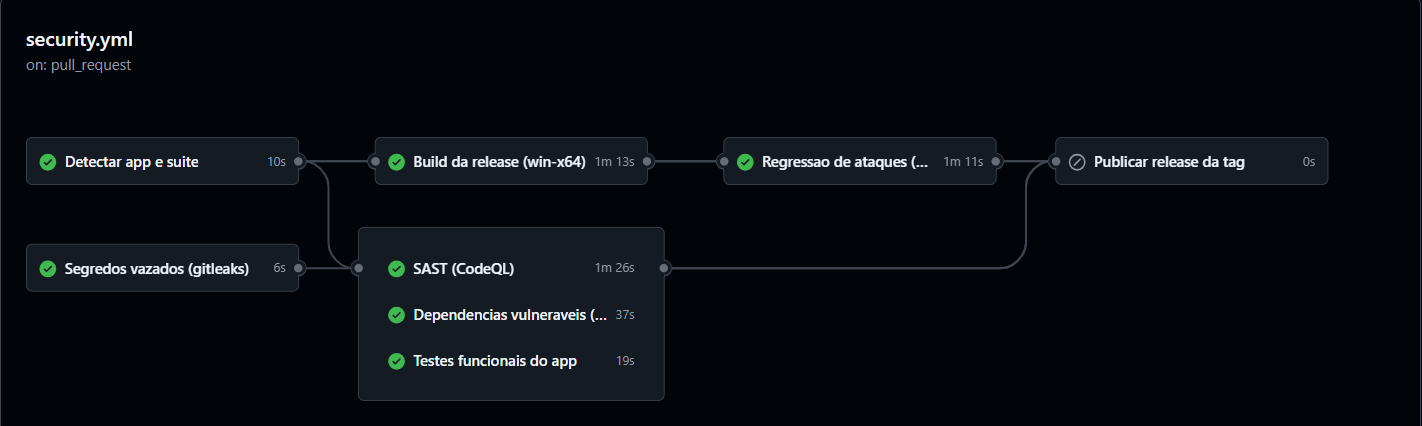
\includegraphics[width=\textwidth]{esteira-run.png}
\caption{Execução da esteira no GitHub Actions para um pull request de documentação (2 min 48 s, verde). A publicação da release só roda em tag.}
\label{fig:esteira}
\end{figure}

A chave privada do fornecedor, necessária para emitir a licença do controle positivo e para assinar o manifesto do pacote, existe na esteira só como o segredo \texttt{NEUROMOCK\_CHAVE\_PRIVADA}, e na máquina do blue fora de qualquer repositório. O risco ficou registrado: um colaborador com permissão de escrita conseguiria ler o segredo por um pull request que alterasse a esteira. Para um trabalho acadêmico, decidiu-se por um segredo simples; no produto real, a chave de emissão ficaria num ambiente com aprovação manual, ou fora da esteira de vez.

Essa organização cobre várias práticas que o CyBOK descreve nos processos prescritivos \parencite{williams2021,howard2006,safecode2018}: análise estática, gestão de componentes de terceiros, uso de ferramentas aprovadas e versões fixadas, e teste de segurança recorrente, adaptado ao DevOps. A gestão de terceiros teve efeito concreto: na v4, a auditoria de dependências barrou um compilador com vulnerabilidade conhecida, como mostra a Seção~\ref{sec:iteracoes}.

\subsection{Medição do custo de ataque}

O custo é a métrica principal do trabalho, por isso foi registrado desde a v0, numa linha por tentativa em \texttt{docs/metricas/custo-ataques.csv}, inclusive as que falharam: uma folha fechada sem tentativa registrada não prova nada. As colunas são data, build, folha, modo, atacante, ferramentas, minutos, resultado e evidência. O modo é \emph{preta}, quando o atacante usou só o artefato da release, ou \emph{branca}, quando consultou o código; o custo só vale para o MATE se o atacante não leu o código, então a caixa branca seria uma segunda medição, registrada à parte. O resultado é sucesso, falha ou timebox.

O timebox é de 2 horas por folha por build, e é um teto, não uma cota: folha que cai em minutos não consome o resto, e o teto só pesa nas que resistem. Ele foi mantido alto de propósito, porque com um teto baixo as builds finais virariam todas \enquote{mais de uma hora} e a curva de custo achataria onde deveria subir. A partir da v2, sucesso passou a ser usar o treino, não só vê-lo abrir: o red registra o resultado depois de deixar o treino aberto por pelo menos um minuto, e a regressão segue a mesma regra. Na árvore 2, o red vence quando entrega uma reimplementação que reproduz a saída do stub num sinal que não viu, e o tempo até lá é o custo.

\subsection{Regras de engajamento e guia do red team}

As regras de engajamento definem o jogo. O red ataca só o zip da release da tag, conferindo o SHA-256; ataca em caixa preta primeiro e só abre \texttt{app/} depois de registrar a tentativa; usa a própria máquina, fiel ao MATE; não ataca a infraestrutura (GitHub, esteira, máquinas dos colegas); e não commita binário adulterado, licença emitida por ele nem segredo, só scripts, passos e hashes.

O guia do red team transforma essas regras num passo a passo para cada ciclo: pegar o alvo e conferir o hash; atacar uma folha por vez dentro do timebox; registrar toda tentativa; abrir uma issue pelo modelo \enquote{Ataque}, com build, SHA-256, folha, modo, passos, evidência, custo e impacto; transformar a issue num teste numa branch \texttt{ataque/<folha>}, rodando a suíte localmente antes do pull request; e levar o resultado à reunião red/blue. O guia traz ainda um bloco de contexto pronto para o assistente de IA do red, que deixa claras as regras de caixa preta e de engajamento, e uma configuração opcional do Claude Code que nega a leitura de \texttt{app/}, para evitar a leitura acidental do código do alvo.

\subsection{Ritmo, ritual e build pronta}

O calendário foi organizado em torno dos encontros presenciais de terça e quinta, com um ciclo por encontro (Quadro~\ref{qd:calendario}). Para caber no prazo, o blue andou uma build à frente: quando o encontro começava, a build seguinte já estava pronta numa branch, e o encontro só consolidava. Se um ciclo atrasasse, a v4 viraria recomendação e a data final não se moveria.

\begin{table}[htbp]
\centering
\caption{Calendário dos ciclos.}
\label{qd:calendario}
\small
\begin{tabular}{L{2.4cm}L{1.4cm}L{1.4cm}L{8.6cm}}
\toprule
Encontro & Fecha & Lança & Testes do red que precisavam estar na \texttt{main} \\
\midrule
qui 05/11 & v0 & v1 & T-F3.1, T-F3.2 e T-F3.3 \\
ter 10/11 & v1 & v2 & T-F1.1, T-F1.2 e T-F1.3 \\
qui 12/11 & v2 & v3 & T-F2.x, T-H1.2 e T-H2.2 \\
ter 17/11 & v3 & v4 & T-H1.1 e T-H2.1 \\
qui 19/11 & v4 & nenhuma & consolidação final; depois, documentação e ensaio \\
\bottomrule
\end{tabular}
\end{table}

Cada encontro tem o mesmo ritual, a reunião red/blue, que é o momento \enquote{purple} do purple teaming: o red mostra o que funcionou, o que não funcionou e quanto custou; os testes do red entram na \texttt{main}; no pull request da build seguinte, as folhas que ela fecha viram \texttt{fechada}; e saem o merge, a coluna da build na matriz, a nota da iteração e a tag. Uma build só é entregue ao red quando a esteira está verde na \texttt{main}, a tag existe e a release foi publicada com o SHA-256, o estado de cada folha está declarado, a coluna da matriz está preenchida e existe a nota da iteração em \texttt{docs/iteracoes/}. Para caber no calendário, valeu ainda uma exceção registrada: se o teste de uma folha atrasasse, o blue podia escrevê-lo a partir dos passos da issue, depois de a tentativa em caixa preta estar registrada, porque a regra de o blue não escrever teste existe só para não revelar o alvo antes do ataque.
